% =========================================================================
% Two Architectures of Cross-Linguality  —  DRAFT-v0 (2026-07-24)
%
% STATUS: DRAFT-v0. Not submitted anywhere. Every number in this file is
% copied from the committed sources of truth in this repository:
%   docs/RESULTS_multilingual_strata.md
%   docs/PREREG_multilingual_strata.md
%   docs/results/strata-multilingual-2026-07-23/*.json
%   docs/results/strata-gutenberg-pair-2026-07-23/*.json
%   docs/HUBNESS_PRIMER.md
% No number appears here that does not appear in (or follow by stated
% arithmetic from) those artifacts.
%
% COMPILATION — honest note: this file uses the ACL style (acl.sty and
% acl_natbib.bst from https://github.com/acl-org/acl-style-files). Those
% files are NOT vendored in this repository; the paper compiles only with
% them present on the TeX path. Figures are self-contained TikZ/pgfplots
% (no external images).
% =========================================================================
\documentclass[11pt]{article}
\usepackage[final]{acl}      % requires acl.sty (not vendored; see header)
\usepackage{times}
\usepackage{latexsym}
\usepackage[T1]{fontenc}
\usepackage[utf8]{inputenc}
\usepackage{microtype}
\usepackage{amsmath}
\usepackage{amssymb}
\usepackage{makecell}
\usepackage{booktabs}
\usepackage{multirow}
\usepackage{xcolor}
\usepackage{tikz}
\usetikzlibrary{arrows.meta,positioning,calc}
\usepackage{pgfplots}
\pgfplotsset{compat=1.18}

% Figure palette (matches the project's other papers' matplotlib palette).
\definecolor{tqblue}{HTML}{1f77b4}
\definecolor{tqred}{HTML}{d62728}
\definecolor{tqgreen}{HTML}{2ca02c}
\definecolor{tqgrey}{HTML}{7f7f7f}
\definecolor{tqorange}{HTML}{ff7f0e}

\newcommand{\draftmark}{\textcolor{tqred}{\textbf{DRAFT-v0}}}
\newcommand{\sk}{S_k}
\newcommand{\tmean}{\bar{\tau}}

\title{Two Architectures of Cross-Linguality:\\
  Trained Interlinguas Dissolve Language Borders;\\
  Emergent Multilinguality Builds a Hub
  \thanks{\draftmark{} --- 2026-07-24. Internal draft; numbers frozen
  against the committed measurement artifacts (see header comment of the
  source). Not for distribution.}}

\author{Andrew H.\ Bond \\
  San Jos\'e State University \\
  \texttt{andrew.bond@sjsu.edu} \\
  ORCID \texttt{0009-0003-2599-6158}}

\begin{document}
\maketitle

\begin{abstract}
Multilingual sentence encoders reach cross-linguality by two routes: an
explicit translation-ranking objective (LaBSE) or emergent alignment from
multilingual pretraining (BGE-M3). We show these routes produce
geometrically distinct architectures of the shared embedding space. Under a
pre-registered protocol with an enforced text-fingerprint replication
predicate, we measure per-language hubness anatomy on 150{,}067 identical
passages in 20 languages encoded by both models. The registered
prediction---that the trained interlingua concentrates cross-lingual
transit in a semantically central ``translationese'' core---inverts on both
legs. LaBSE produces \emph{more} transit (mean transit fraction 0.389 vs.\
0.291), carried by rows \emph{less} central than the population
($-0.0086$, $p=1.0$), spread \emph{less} concentratedly across languages
(top-3 share 0.391 vs.\ 0.473; Gini 0.508 vs.\ 0.574), and turns seven of
thirteen eligible languages into backbone-class areas. BGE-M3 keeps every
language in the local-hub (NSHA) class and routes its smaller transit
through a central hub region ($+0.0041$, $p<10^{-4}$). In short: training
an interlingua does not build a translationese core---it dissolves the
language borders; emergent multilinguality keeps the borders and routes
traffic through a hub. Two further frozen predictions also resolved
against us, and we report them as findings: BGE-M3 \emph{homogenizes}
per-language hubness (a Robin Hood band of width 0.10 across 7 languages,
3 scripts, and $\sim$3 millennia of text), and compression damage at a
deployed $27.676\times$ operating point orders near-monotonically by
resource level---the three worst anti-hub strata are exactly the three
lowest-resource languages---while staying below the registered effect size
and invisible to aggregate recall (0.8233). All predictions were frozen
before measurement; confirmations and embarrassments are typeset
identically. We argue this reporting contract is itself a contribution.
\end{abstract}

\section{Introduction}
\label{sec:intro}

How does a multilingual embedding space organize its languages? Two
training regimes dominate: \emph{trained} interlinguas, where a
translation-ranking objective explicitly pulls parallel sentences together
\cite{feng2022labse}, and \emph{emergent} multilinguality, where alignment
arises as a side effect of multilingual pretraining and distillation
\cite{chen2024bgem3}. A natural hypothesis---the one we pre-registered---is
that the explicit objective builds a \emph{stronger} version of the same
structure: a semantically central, translationese-like core through which
cross-lingual neighbor traffic concentrates.

That hypothesis is wrong, and wrong in an informative direction. Measured
with per-language hubness instruments on 150{,}067 \emph{identical}
passages encoded by both models---identity enforced by a text-fingerprint
replication predicate that refuses, rather than warns on, mismatched
inputs---the two regimes produce two different \emph{architectures}
(Fig.~\ref{fig:architectures}):

\begin{itemize}
\item \textbf{Emergent (BGE-M3): borders plus a hub.} Every eligible
language classifies as a not-so-hubby area (NSHA: strong local hubs, low
global transit). Cross-lingual transit is comparatively scarce (mean
transit fraction $\tmean = 0.291$), concentrated in a few languages
(top-3 share 0.473, Gini 0.574), and carried by rows \emph{more}
semantically central than the population ($+0.0041$, one-sided permutation
$p < 10^{-4}$).
\item \textbf{Trained (LaBSE): borders dissolved.} Transit is more
abundant ($\tmean = 0.389$; at least 10\% of rows are pure transit,
$\tau = 1.0$), more evenly spread (top-3 share 0.391, Gini 0.508), carried
by rows \emph{less} central than the population ($-0.0086$, $p = 1.0$),
and seven of thirteen eligible languages become \emph{backbone-class}
areas---the first backbone-class areas these instruments have measured.
\end{itemize}

This paper reports that inversion (P2) as its headline, together with two
companion registered predictions that also failed, each failure a finding:

\textbf{P1 (heterogeneity--- failed; homogenization found).} We predicted
per-language hubness would vary widely under BGE-M3. Instead, seven
languages spanning $63\times$ in sample size, three scripts, and roughly
three millennia of text land in a Robin Hood band of width 0.10
(\S\ref{sec:p1}).

\textbf{P3 (concentrated compression damage--- sub-threshold; ordering
found).} At the deployed $27.676\times$ compression operating point,
per-language anti-hub recall orders near-monotonically by resource level,
and the bottom-3 strata are exactly the three lowest-resource languages,
while aggregate recall reads green (0.8233). The registered 0.10 gap was
\emph{not} met (measured 0.088, resp.\ 0.058 under the two declared
readings), so we label the result exactly what it is: a directional,
sub-registered-threshold finding with direct equity implications for
low-resource retrieval (\S\ref{sec:p3}).

\textbf{Methodology as contribution.} All predictions were frozen in a
pre-registration before any stratified measurement existed (content hash
in \S\ref{sec:design}); operationalizations could only tighten; the
results document typesets confirmations and embarrassments identically,
and this paper reproduces its scoreboard verbatim
(\S\ref{sec:methodology}). Two of two registered mechanism predictions
were falsified by our own instruments---which we take as the strongest
available evidence that the instruments were worth building.

\section{Background: Hubness, Per-Language Anatomy, and Transit}
\label{sec:background}

\textbf{Hubness.} In high-dimensional spaces, $k$-nearest-neighbor
relations are asymmetric: a few points (\emph{hubs}) appear in very many
top-$k$ lists while a large fraction (\emph{anti-hubs}) appear in almost
none \cite{radovanovic2010hubs}. For each row $x$, write $N_k(x)$ for the
number of queries whose top-$k$ contains $x$. Hubness is a property of the
(corpus, query distribution, metric, $k$) experiment, not of the corpus
alone. Because the skewness of $N_k$ grows with $n$, cross-population
comparisons use size-stable statistics: the \emph{Robin Hood index} (the
share of counts that would have to move to equalize the distribution) and
\emph{frac\_above\_2k} (the fraction of rows with $N_k > 2k$)
\cite{feldbauer2020scikit}. Hubness correction is a standard tool in
cross-lingual retrieval, e.g.\ CSLS \cite{conneau2018word}; it has also
become an attack surface---centroid-seeking vector injections
(\emph{black-hole} attacks) exploit centrality-driven hubness
\cite{blackhole2026}, and open-source scanners detect hubness poisoning
via count outliers and cross-cluster retrieval spread \cite{advhubness2026}.

\textbf{Per-language anatomy.} We partition the corpus into
\emph{areas} (here: languages) and split each row's count into intra-area
and transit components: $\tau(x)$ is the fraction of $x$'s appearances in
top-$k$ lists of queries from \emph{other} areas. Per area we report count
skew $\sk$, $\max N_k$, mean transit $\tmean$, Robin Hood index,
frac\_above\_2k, and Spearman correlations of count with local density
($-d_k$) and centrality. Areas classify by report-carried thresholds
($\theta_\tau = 0.5$, $\theta_N = 50$ here): a \emph{backbone} area has
$\tmean \ge \theta_\tau$ with $\max N_k \ge \theta_N$ (its hubs are
cross-lingual transit); an \emph{NSHA} (``not-so-hubby area'') has strong
local hubs but low global transit---each language its own hub economy.

\textbf{Anti-hub recall.} Queries whose true nearest neighbors are
anti-hubs are the hardest retrieval cases, and quantization damages them
first while aggregate recall barely moves. \emph{Anti-hub recall} is
recall restricted to queries whose true nearest neighbor lies in the
bottom count decile; the project's operating rule is ``trust the tail,
not the mean.''

\section{Experimental Design}
\label{sec:design}

\subsection{Pre-registration}
All predictions (P1--P4) were frozen on 2026-07-23, before any stratified
measurement existed, in a pre-registration whose content hash the results
document cites: SHA-256
\texttt{5c6f74f7cfa3cdf6539ed1fb10a938a37a6ebd2f0def46b835d4d668022d4b55}
(the file as committed at \texttt{3b02ae6}). The amendment rule permits
only \emph{tightening} of operationalizations, with dated changelog
entries, never after seeing results for the statistic in question. No
amendments to the prediction section were made.

\subsection{Corpora and arms}
\label{sec:corpora}

\textbf{Arm A (P1, P3, P4): Ethics corpus, BGE-M3.} 2{,}391{,}361
embedded rows (1024-d) carrying 40 language labels (the pre-registration's
materials table said 37; the measured count governs). A uniform sample of
$N = 350{,}000$ rows (seed 7) preserves the corpus measure; per-language
$n$ falls where it falls. Seven of 14 labeled strata are eligible
($n \ge n_{\min} = 2000$): Hebrew 134{,}524; Aramaic 123{,}820; English
44{,}929; Greek 32{,}289; Latin 7{,}038; Sanskrit 4{,}780; Pali 2{,}132.
Seven ABSTAIN (\S\ref{sec:p4}).

\textbf{Paired Gutenberg rung (P2): both encoders on identical texts.}
150{,}067 passages in 20 languages (13 with $n \ge 2000$; a deliberate
ABSTAIN tail), deterministically extracted (seed 7, paragraph-pack
400--900 characters, $\le 40$ per book, public mirror), each row carrying
a text SHA-256. Encoded by \texttt{BAAI/bge-m3} (1024-d) and
\texttt{sentence-transformers/LaBSE} (768-d) with the identical
\texttt{sentence-transformers} invocation
(\texttt{normalize\_embeddings=True}).

\textbf{The replication predicate (refuse $\ne$ warn).} The P2 encoder
contrast is only scored where both arms' metadata carry the identical
order-sensitive corpus text fingerprint
(\texttt{f3e19747c0e6af39feb06017ac6fa6b131a7f03fcc975ab2efe6a689de46b0cf}),
enforced \emph{in the scoring script}: on mismatch it refuses to emit a
comparison rather than warning. This predicate did real work: the original
1M-row LaBSE rung had no recoverable row$\to$text mapping, so the
comparison against it was refused and the paired rung above was built to
replace it (a dated, discipline-tightening materials changelog entry;
prediction text untouched).

\subsection{Protocol}
Exact $k$NN on the given unit-normalized vectors ($k = 10$; Euclidean rank
$\equiv$ cosine rank), corpus$\to$corpus battery (declared primary;
hubness depends on who is asking). Thresholds $n_{\min} = 2000$,
$q_{\min} = 500$, $\theta_\tau = 0.5$, $\theta_N = 50$; all are fields of
the report artifacts, not constants. Correlations are Spearman. P3 runs at
the deployed compression operating point: PCA-384 + TQ3, measured
$27.676\times$, single-pass ADC, no rerank, build seed 42. Software:
turboquant-pro 2.0.0a2 + STRATA Phase-1 (\texttt{209902f}). All artifacts
(anatomy reports, hubdiff reports, P2 score; no vectors, no text) are
committed beside the results document.

\begin{figure*}[t]
\centering
\resizebox{\textwidth}{!}{%
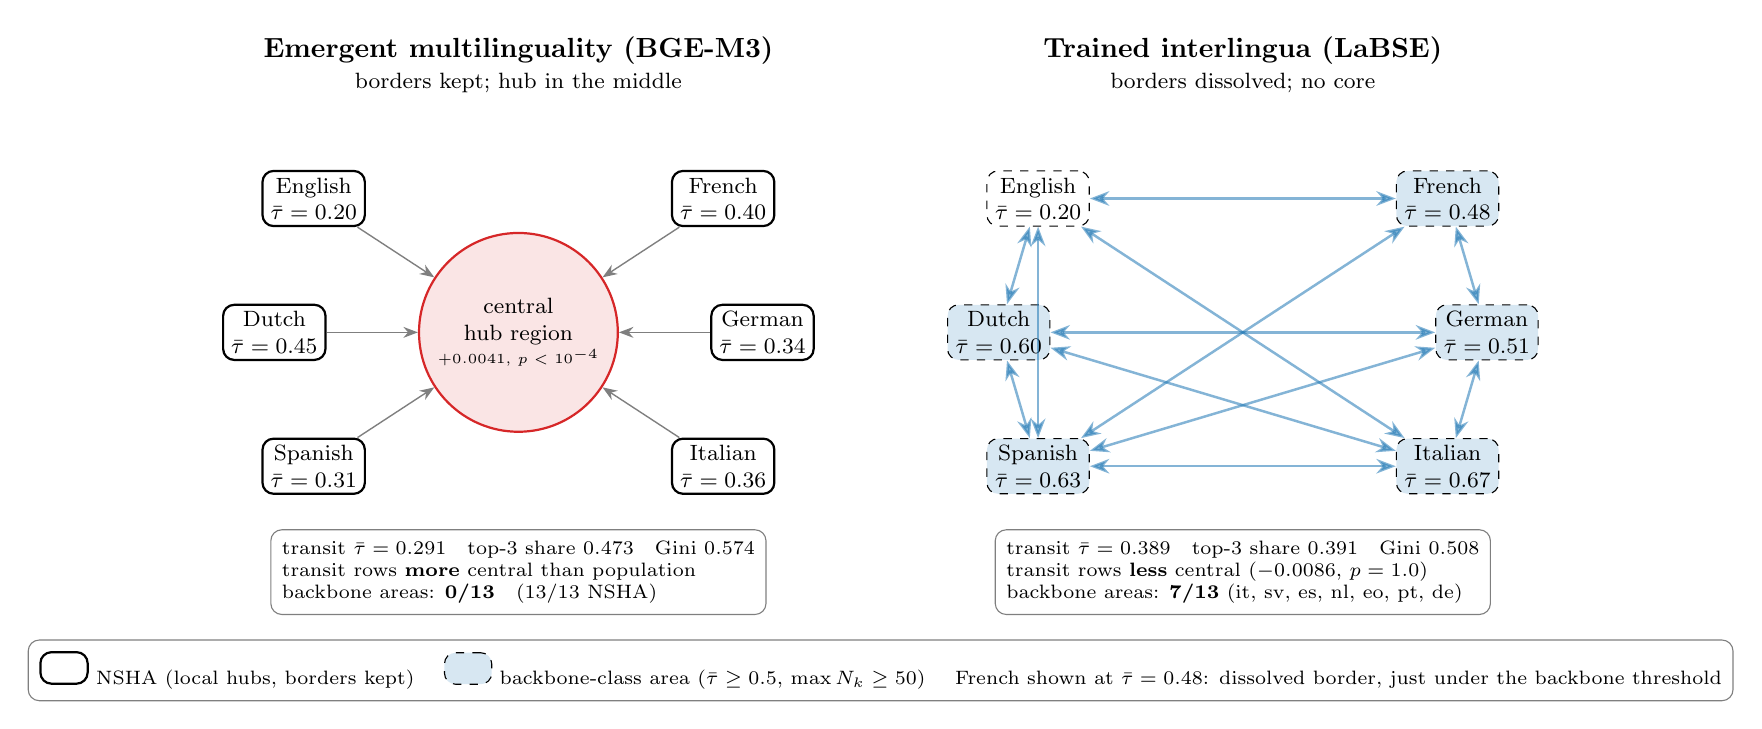
\begin{tikzpicture}[
  font=\footnotesize,
  lang/.style={draw, rounded corners, align=center, minimum width=13mm,
               minimum height=7mm, inner sep=2pt},
  nsha/.style={lang, thick, fill=white},
  bb/.style={lang, dashed, fill=tqblue!18},
  dis/.style={lang, dashed, fill=white},
  hubcore/.style={draw=tqred, thick, fill=tqred!12, circle,
                  minimum size=17mm, align=center},
  note/.style={draw=tqgrey, rounded corners, align=left, inner sep=4pt,
               font=\scriptsize},
  >={Stealth[]}]

% ---------------- Left panel: EMERGENT (BGE-M3) ----------------
\begin{scope}[local bounding box=left]
\node[font=\normalsize\bfseries, align=center] at (0, 3.4)
  {Emergent multilinguality (BGE-M3)\\[-1pt]
   \normalfont\footnotesize borders kept; hub in the middle};
\node[hubcore] (core) at (0,0)
  {central\\hub region\\[-1pt]{\tiny $+0.0041$, $p<10^{-4}$}};
\node[nsha] (en)  at (-2.6,  1.7) {English\\$\tmean=0.20$};
\node[nsha] (fr)  at ( 2.6,  1.7) {French\\$\tmean=0.40$};
\node[nsha] (nl)  at (-3.1,  0.0) {Dutch\\$\tmean=0.45$};
\node[nsha] (de)  at ( 3.1,  0.0) {German\\$\tmean=0.34$};
\node[nsha] (es)  at (-2.6, -1.7) {Spanish\\$\tmean=0.31$};
\node[nsha] (it)  at ( 2.6, -1.7) {Italian\\$\tmean=0.36$};
\foreach \l in {en,fr,nl,de,es,it}{
  \draw[->, tqgrey, line width=0.5pt] (\l) -- (core);}
\node[note, anchor=north] at (0,-2.5)
  {transit $\tmean = 0.291$ \; top-3 share $0.473$ \; Gini $0.574$\\
   transit rows \textbf{more} central than population\\
   backbone areas: \textbf{0/13} \; (13/13 NSHA)};
\end{scope}

% ---------------- Right panel: TRAINED (LaBSE) ----------------
\begin{scope}[shift={(9.2,0)}, local bounding box=right]
\node[font=\normalsize\bfseries, align=center] at (0, 3.4)
  {Trained interlingua (LaBSE)\\[-1pt]
   \normalfont\footnotesize borders dissolved; no core};
\node[dis] (ren)  at (-2.6,  1.7) {English\\$\tmean=0.20$};
\node[bb]  (rfr)  at ( 2.6,  1.7) {French\\$\tmean=0.48$};
\node[bb]  (rnl)  at (-3.1,  0.0) {Dutch\\$\tmean=0.60$};
\node[bb]  (rde)  at ( 3.1,  0.0) {German\\$\tmean=0.51$};
\node[bb]  (res)  at (-2.6, -1.7) {Spanish\\$\tmean=0.63$};
\node[bb]  (rit)  at ( 2.6, -1.7) {Italian\\$\tmean=0.67$};
% diffuse pairwise transit, no central node
\foreach \a/\b in {ren/rfr, ren/rnl, rfr/rde, rnl/res, rde/rit, res/rit,
                   rnl/rde, res/rfr, ren/rit, rnl/rit, res/rde, ren/res}{
  \draw[<->, tqblue, line width=0.9pt, opacity=0.55] (\a) -- (\b);}
\node[note, anchor=north] at (0,-2.5)
  {transit $\tmean = 0.389$ \; top-3 share $0.391$ \; Gini $0.508$\\
   transit rows \textbf{less} central ($-0.0086$, $p=1.0$)\\
   backbone areas: \textbf{7/13} (it, sv, es, nl, eo, pt, de)};
\end{scope}

% legend between panels
\node[note, anchor=north] at (4.6, -3.9)
  {\tikz{\node[nsha, minimum width=6mm, minimum height=4mm]{};} NSHA
   (local hubs, borders kept) \quad
   \tikz{\node[bb, minimum width=6mm, minimum height=4mm]{};}
   backbone-class area ($\tmean \ge 0.5$, $\max N_k \ge 50$) \quad
   French shown at $\tmean=0.48$: dissolved border, just under the
   backbone threshold};
\end{tikzpicture}}
\caption{The two architectures of cross-linguality, measured on the same
150{,}067 passages (six of the 13 eligible languages drawn; all per-language
$\tmean$ values from the committed anatomy reports, panel summary statistics
from the committed P2 score). \emph{Left:} under emergent multilinguality
(BGE-M3) every eligible language keeps its border (13/13 NSHA, 0 backbone);
the smaller transit mass ($\tmean = 0.291$) concentrates in few languages
(top-3 share 0.473, Gini 0.574) and is carried by rows \emph{more}
semantically central than the population ($+0.0041$, one-sided permutation
$p < 10^{-4}$)---a hub region in the middle of the space. \emph{Right:}
the trained translation-ranking objective (LaBSE) dissolves the borders:
more transit ($\tmean = 0.389$), spread more evenly (top-3 share 0.391,
Gini 0.508), carried by rows \emph{less} central than the population
($-0.0086$, $p = 1.0$), with seven of thirteen languages becoming
backbone-class areas (Italian 0.67, Swedish 0.65, Spanish 0.63, Dutch
0.60, Esperanto 0.58, Portuguese 0.57, German 0.51). The registered
prediction expected the left-hand structure, only stronger, on the right.}
\label{fig:architectures}
\end{figure*}

\section{P2: The Inversion---Trained Interlinguas Dissolve Borders}
\label{sec:p2}

\textbf{Registered prediction.} Cross-lingual transit concentrates in a
semantically central (translationese) region, \emph{more strongly} under
LaBSE than under BGE-M3. Operationalized before measurement, with strict
readings fixed in the scoring script's docstring: (i) top-decile-$\tau$
rows have mean centrality above the population (one-sided permutation
test, 10{,}000 permutations, seed 7, $\alpha = 0.01$, must hold in
\emph{both} arms); (ii) transit concentration (top-3-language share of
top-decile-$\tau$ mass, and its Gini) strictly higher for LaBSE. Both
required for \emph{confirmed}; (i) alone = partial.

\textbf{Verdict: NOT CONFIRMED---the sign flipped on both legs.}
Table~\ref{tab:p2} reproduces the scoreboard from the results document
verbatim.

\begin{table}[t]
\centering
\small
\setlength{\tabcolsep}{3.5pt}
\begin{tabular}{lccc}
\toprule
statistic & \makecell{BGE-M3\\(emergent)} & \makecell{LaBSE\\(trained)} &
  \makecell{registered\\direction} \\
\midrule
overall mean $\tau$ & 0.291 & \textbf{0.389} & --- \\
top-decile-$\tau$ threshold & 0.75 & \textbf{1.00} & --- \\
\makecell[l]{(i) centrality diff\\ \quad of top-$\tau$ rows} &
  \makecell{\textbf{+0.0041}\\$p<10^{-4}$ \checkmark} &
  \makecell{$-0.0086$\\$p=1.0$ $\times$} & above pop. \\
(ii) share\_top3 & \textbf{0.473} & 0.391 & LaBSE higher $\times$ \\
(ii) Gini of transit mass & \textbf{0.574} & 0.508 & LaBSE higher $\times$ \\
\bottomrule
\end{tabular}
\caption{P2 scoreboard, reproduced from the results document. For LaBSE
the top-decile-$\tau$ threshold saturates at 1.00: at least 10\% of all
rows are \emph{pure transit} (every top-$k$ appearance from another
language). Registered verdict: NOT CONFIRMED, inverted on both legs.}
\label{tab:p2}
\end{table}

\begin{table}[t]
\centering
\small
\setlength{\tabcolsep}{4pt}
\begin{tabular}{lrcccc}
\toprule
 & & \multicolumn{2}{c}{BGE-M3} & \multicolumn{2}{c}{LaBSE} \\
\cmidrule(lr){3-4}\cmidrule(lr){5-6}
language & $n$ & $\tmean$ & class & $\tmean$ & class \\
\midrule
English    & 60{,}000 & 0.196 & NSHA & 0.200 & NSHA \\
French     & 15{,}000 & 0.398 & NSHA & 0.484 & NSHA \\
Finnish    & 15{,}000 & 0.323 & NSHA & 0.394 & NSHA \\
German     & 15{,}000 & 0.336 & NSHA & 0.511 & \textbf{backbone} \\
Dutch      & 10{,}000 & 0.453 & NSHA & 0.603 & \textbf{backbone} \\
Spanish    & 10{,}000 & 0.306 & NSHA & 0.625 & \textbf{backbone} \\
Italian    &  6{,}615 & 0.364 & NSHA & 0.668 & \textbf{backbone} \\
Greek      &  4{,}000 & 0.185 & NSHA & 0.384 & NSHA \\
Hungarian  &  3{,}985 & 0.417 & NSHA & 0.493 & NSHA \\
Esperanto  &  2{,}332 & 0.361 & NSHA & 0.582 & \textbf{backbone} \\
Latin      &  2{,}189 & 0.293 & NSHA & 0.398 & NSHA \\
Portuguese &  2{,}103 & 0.415 & NSHA & 0.571 & \textbf{backbone} \\
Swedish    &  2{,}000 & 0.437 & NSHA & 0.650 & \textbf{backbone} \\
\midrule
\multicolumn{2}{l}{backbone count} & \multicolumn{2}{c}{\textbf{0/13}} &
  \multicolumn{2}{c}{\textbf{7/13}} \\
\bottomrule
\end{tabular}
\caption{Per-language anatomy on the paired Gutenberg rung (identical
texts, both encoders; values from the committed per-arm anatomy reports,
$\tmean$ to three decimals). Under BGE-M3 all thirteen eligible languages
are NSHA. Under LaBSE seven cross the backbone predicate
($\tmean \ge 0.5$, $\max N_k \ge 50$)---the first backbone-class areas
these instruments have measured. Seven further strata ABSTAIN in both arms
(\S\ref{sec:p4}).}
\label{tab:p2anatomy}
\end{table}

\textbf{Reading the inversion.} The registered thesis conflated
``stronger interlingua'' with ``more concentrated transit,'' and the
measurement pulls them apart. The translation-ranking objective produces
\emph{more} cross-lingual transit overall ($\tmean$ 0.389 vs.\ 0.291),
carried by rows \emph{less} central than the population, spread
\emph{less} concentratedly across languages---and, per the stratified
anatomy (Table~\ref{tab:p2anatomy}), it turns seven of thirteen eligible
languages into backbone-class areas. Emergent multilinguality is the
opposite architecture: less transit, concentrated in a semantically
central region (leg (i) holds \emph{only} there), and zero backbone
areas---all thirteen strata NSHA. Training an interlingua does not build a
translationese core; it dissolves the language borders. Emergent
multilinguality keeps the borders and routes traffic through a hub region.

Note what makes the comparison licit: both arms encode the byte-identical
row list (fingerprint match enforced; \S\ref{sec:corpora}), the same
battery, the same $k$, the same thresholds. The dimensionality difference
(1024 vs.\ 768) is declared, not hidden.

\section{P1: BGE-M3 Homogenizes Per-Language Hubness}
\label{sec:p1}

\textbf{Registered prediction.} Among non-ABSTAIN languages of the Ethics
corpus (arm A), per-language hubness varies widely: max/min Robin Hood
ratio $\ge 1.5$ \emph{and} max/min $\sk$ ratio $\ge 3$. The registered
fallback: ``if it fails: the encoder homogenizes geometry across languages
far more than expected---itself a publishable finding about BGE-M3, and
the reviewer eats it publicly.''

\textbf{Verdict: NOT CONFIRMED; the fallback stands as the finding.}
Measured: Robin Hood 0.3447 (English) \ldots{} 0.4469 (Sanskrit), ratio
$\mathbf{1.30} < 1.5$; $\sk$ 2.68 (English) \ldots{} 4.40 (Greek), ratio
$\mathbf{1.64} < 3$. Both legs fail. The pre-committed cross-size rule was
honored: Robin Hood primary, $\sk$ printed beside per-stratum $n$.

\begin{table}[t]
\centering
\small
\setlength{\tabcolsep}{3pt}
\begin{tabular}{lrccccc}
\toprule
language & $n$ & $\sk$ & $\max N_k$ & $\tmean$ & RH & class \\
\midrule
Hebrew   & 134{,}524 & 3.84 & 247 & 0.214  & 0.385 & NSHA \\
Aramaic  & 123{,}820 & 4.21 & 287 & 0.302  & 0.357 & NSHA \\
English  &  44{,}929 & 2.68 & 163 & 0.189  & 0.345 & NSHA \\
Greek    &  32{,}289 & 4.40 & 280 & 0.074  & 0.398 & NSHA \\
Latin    &   7{,}038 & 3.86 & 188 & 0.185  & 0.420 & NSHA \\
Sanskrit &   4{,}780 & 3.97 & 229 & 0.0024 & 0.447 & NSHA \\
Pali     &   2{,}132 & 4.22 & 157 & 0.0004 & 0.386 & NSHA \\
\bottomrule
\end{tabular}
\caption{P1: per-language anatomy of the Ethics corpus under BGE-M3
(uniform 350{,}000-row sample, seed 7; values from the committed anatomy
report; RH = Robin Hood index). Seven languages spanning $63\times$ in
sample size, three scripts, and $\sim$3 millennia of text land in a Robin
Hood band of width 0.10, and all classify NSHA.}
\label{tab:p1}
\end{table}

\begin{figure}[t]
\centering
\resizebox{\columnwidth}{!}{%
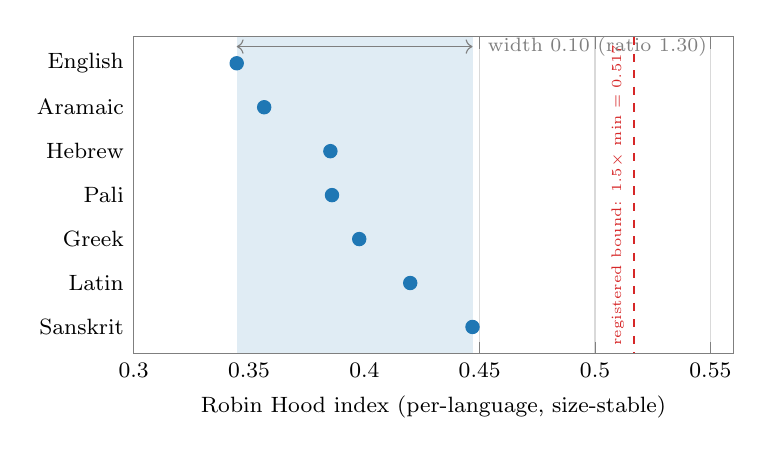
\begin{tikzpicture}
\begin{axis}[
  font=\footnotesize,
  width=9.2cm, height=5.6cm,
  xlabel={Robin Hood index (per-language, size-stable)},
  xmin=0.30, xmax=0.56,
  ytick={1,...,7},
  yticklabels={English, Aramaic, Hebrew, Pali, Greek, Latin, Sanskrit},
  y dir=reverse, ymin=0.4, ymax=7.6,
  ytick style={draw=none},
  xmajorgrids, grid style={tqgrey!30},
  axis line style={tqgrey},
  clip=false,
]
% measured band [min, max] = [0.3447, 0.4469], width 0.10
\fill[tqblue!14] (axis cs:0.3447,0.4) rectangle (axis cs:0.4469,7.6);
\addplot[only marks, mark=*, mark size=2.4pt, tqblue] coordinates {
  (0.3447,1) (0.3566,2) (0.3853,3) (0.3860,4) (0.3978,5) (0.4199,6)
  (0.4469,7)};
% registered confirmation bound: 1.5 x min = 0.517 (stated arithmetic)
\draw[tqred, dashed, thick] (axis cs:0.517,0.4) -- (axis cs:0.517,7.6)
  node[pos=0.5, rotate=90, above, font=\tiny\color{tqred}, align=center]
  {registered bound: $1.5\times$ min $= 0.517$};
\draw[<->, tqgrey] (axis cs:0.3447,0.62) -- (axis cs:0.4469,0.62)
  node[right, font=\scriptsize, xshift=2pt]
  {width 0.10 (ratio 1.30)};
\end{axis}
\end{tikzpicture}}
\caption{P1: the homogenization band. Per-language Robin Hood indices of
the seven eligible Ethics strata under BGE-M3 (dots; values in
Table~\ref{tab:p1}) span only 0.3447--0.4469: a band of width 0.10, ratio
1.30. The registered heterogeneity prediction required the maximum to
reach $1.5\times$ the minimum ($= 0.517$, dashed line, computed from the
registered ratio and the measured minimum)---no language comes close. The
secondary leg fails likewise ($\sk$ ratio 1.64 $< 3$).}
\label{fig:p1band}
\end{figure}

Seven languages spanning $63\times$ in sample size, three scripts, and
roughly three millennia of text land in a Robin Hood band of width 0.10
(Fig.~\ref{fig:p1band}), and all seven classify NSHA. Where the languages
\emph{do} differ is transit: $\tmean$ spans Aramaic 0.302 $>$ Hebrew 0.214
$>$ English 0.189 $>$ Latin 0.185 $>$ Greek 0.074 $\gg$ Sanskrit 0.0024
$>$ Pali 0.0004 (exploratory; the Hebrew--Aramaic pair, drawn from
mixed-language corpora, shows an order of magnitude more cross-language
neighbor traffic than the hermetically self-contained Indic strata).
Mechanism evidence is density-flavored throughout:
$\mathrm{corr}(\mathrm{count}, -d_k)$ 0.48--0.76 with
$\mathrm{corr}(\mathrm{count}, \mathrm{centrality})$ 0.14--0.35 across
strata; no centrality-artifact signature in any stratum (per doctrine,
non-gating).

\section{P3: Compression Damage Orders by Resource Level While Aggregate
Recall Reads Green}
\label{sec:p3}

\textbf{Registered prediction (directional, weaker prior).} At the
deployed $27.676\times$ operating point (PCA-384 + TQ3, single-pass ADC,
no rerank), min-over-strata anti-hub recall is at least 0.10 below the
aggregate; worst strata among low-resource languages; aggregate in its
green band.

\textbf{Verdict: NOT CONFIRMED at the registered threshold.} Aggregate
recall@10 \textbf{0.8233} (p05 0.60); aggregate anti-hub recall
\textbf{0.7933}; min-over-strata anti-hub recall \textbf{0.7355}
(Sanskrit). The gap is \textbf{0.088} against aggregate recall@10 and
\textbf{0.058} against aggregate anti-hub recall---under \emph{either}
declared reading of ``the aggregate,'' below the registered 0.10. No
post-hoc reading selection: both are reported, both fail.

\begin{table}[t]
\centering
\small
\setlength{\tabcolsep}{4pt}
\begin{tabular}{lrccc}
\toprule
language & $n_q$ & recall@10 & p05 & anti-hub \\
\midrule
English  &  44{,}929 & 0.8434 & 0.7 & 0.8110 \\
Aramaic  & 123{,}820 & 0.8378 & 0.6 & 0.8041 \\
Hebrew   & 134{,}524 & 0.8140 & 0.6 & 0.7874 \\
Greek    &  32{,}289 & 0.7971 & 0.6 & 0.7793 \\
Pali     &   2{,}132 & 0.7998 & 0.6 & \textbf{0.7758} \\
Latin    &   7{,}038 & 0.7845 & 0.6 & \textbf{0.7733} \\
Sanskrit &   4{,}780 & 0.7613 & 0.6 & \textbf{0.7355} \\
\midrule
aggregate & 350{,}000 & 0.8233 & 0.60 & 0.7933 \\
\bottomrule
\end{tabular}
\caption{P3: per-language retrieval under the deployed $27.676\times$
compression operating point (values from the committed hubdiff reports;
rows ordered by resource level as in the results document). The bottom-3
anti-hub strata (bold) are exactly the three lowest-resource eligible
languages. All seven strata carry verdict \emph{fail} with registered
cause \texttt{stratum\_anti\_hub\_gap} at the demonstration gate
(\texttt{--min-anti-recall 0.90}).}
\label{tab:p3}
\end{table}

\begin{figure}[t]
\centering
\resizebox{\columnwidth}{!}{%
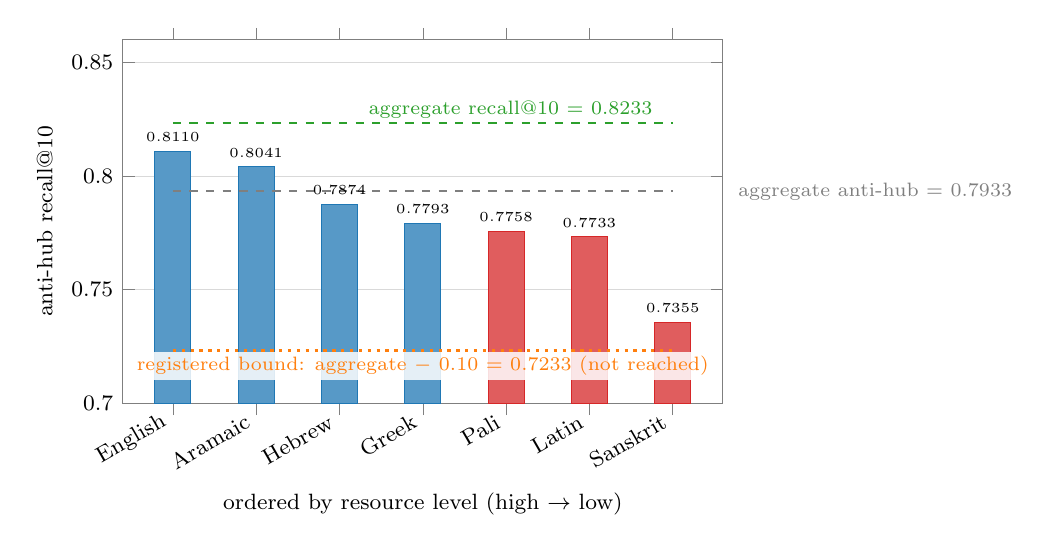
\begin{tikzpicture}
\begin{axis}[
  font=\footnotesize,
  width=9.2cm, height=6.2cm,
  ybar=0pt, bar width=13pt, bar shift=0pt,
  ylabel={anti-hub recall@10},
  ymin=0.70, ymax=0.86,
  symbolic x coords={English,Aramaic,Hebrew,Greek,Pali,Latin,Sanskrit},
  xtick={English,Aramaic,Hebrew,Greek,Pali,Latin,Sanskrit},
  x tick label style={rotate=30, anchor=east},
  xlabel={ordered by resource level (high $\to$ low)},
  ymajorgrids, grid style={tqgrey!30},
  axis line style={tqgrey},
  nodes near coords, nodes near coords style={font=\tiny},
  every node near coord/.append style={/pgf/number format/.cd,
    fixed, fixed zerofill, precision=4},
  clip=false,
]
\addplot[fill=tqblue!75, draw=tqblue] coordinates {
  (English,0.8110) (Aramaic,0.8041) (Hebrew,0.7874) (Greek,0.7793)};
\addplot[fill=tqred!75, draw=tqred] coordinates {
  (Pali,0.7758) (Latin,0.7733) (Sanskrit,0.7355)};
\draw[tqgreen, dashed, thick]
  (axis cs:English,0.8233) -- (axis cs:Sanskrit,0.8233)
  node[pos=0.97, above left, font=\scriptsize\color{tqgreen},
       fill=white, fill opacity=0.85, text opacity=1, inner sep=1.5pt]
  {aggregate recall@10 = 0.8233};
\draw[tqgrey, dashed, thick]
  (axis cs:English,0.7933) -- (axis cs:Sanskrit,0.7933);
\node[anchor=west, font=\scriptsize\color{tqgrey}, xshift=2pt]
  at ({rel axis cs:1,0}|-{axis cs:English,0.7933})
  {aggregate anti-hub = 0.7933};
\draw[tqorange, dotted, very thick]
  (axis cs:English,0.7233) -- (axis cs:Sanskrit,0.7233)
  node[pos=0.5, below, font=\scriptsize\color{tqorange},
       fill=white, fill opacity=0.85, text opacity=1, inner sep=1.5pt]
  {registered bound: aggregate $-$ 0.10 $=$ 0.7233 (not reached)};
\end{axis}
\end{tikzpicture}}
\caption{P3: the damage ordering. Per-language anti-hub recall at the
deployed $27.676\times$ operating point, languages ordered by resource
level (values from Table~\ref{tab:p3}). Damage orders near-monotonically
with resource level, and the bottom-3 strata (red) are exactly the three
lowest-resource eligible languages---while aggregate recall@10 (green
dashed) reads 0.8233. The registered confirmation bound (aggregate
$-$ 0.10 $=$ 0.7233, dotted; arithmetic from the registered threshold and
the measured aggregate) is \emph{not} reached: minimum 0.7355, gap 0.088.
The finding is directional and sub-registered-threshold, and is labeled
exactly so.}
\label{fig:p3damage}
\end{figure}

\textbf{The sub-threshold finding.} The \emph{directional} component did
land, and is recorded as exploratory (sub-threshold, not a confirmation):
the bottom-3 anti-hub strata---Sanskrit 0.7355, Latin 0.7733, Pali
0.7758---are exactly the three lowest-resource eligible languages, and
per-stratum anti-hub recall orders near-monotonically with resource level
(English 0.8110 $>$ Aramaic 0.8041 $>$ Hebrew 0.7874 $>$ Greek 0.7793 $>$
Pali 0.7758 $>$ Latin 0.7733 $>$ Sanskrit 0.7355;
Fig.~\ref{fig:p3damage}). A magnitude-honest summary: the damage
concentration is real but roughly half the registered effect size at this
operating point.

\textbf{Equity implication.} A deployment gating only on aggregate recall
would ship this index: 0.8233 looks green. The languages paying for the
compression are the ones least represented---an equity failure mode that
per-stratum gating catches and aggregate gating structurally cannot. As
tooling (not a registered claim): at \texttt{--min-anti-recall 0.90}, all
7 eligible strata fail and the gate exits 1---the min-over-strata gate
fires on real production-shaped data.

\textbf{Green-band caveat, stated plainly.} This run used the single-pass
ADC path (no rerank), declared in provenance. Historical single-pass
readings in this project (e.g.\ 0.592 ADC-only at a 1B-row run on a
different corpus) are not a calibrated band for this corpus; the
per-stratum \emph{contrast} is the pre-registered object, measured under
one fixed operating point for all strata.

\section{P4: ABSTAIN Is a Result}
\label{sec:p4}

The registered expectation that real data would exercise the
minimum-evidence path was confirmed: 7 of 14 Ethics strata ABSTAIN with
registered cause \texttt{stratum\_insufficient\_n} (Old Norse/English 336,
Arabic 112, Classical Chinese 35, Tamil 2, French/Georgian/Indonesian 1
each), excluded from gating, reported and counted; likewise 7 of 20
Gutenberg strata in both arms (Chinese 984, Japanese 291, Polish 312,
Hebrew 120, Czech 80, Russian 46, Persian 10). A stratum below
$n_{\min} = 2000$ rows or $q_{\min} = 500$ queries yields no verdict rather
than a noisy one. We highlight this because the alternative---silently
folding tail languages into an aggregate---is precisely the failure mode
P3 documents.

\section{The Reporting Contract as a Contribution}
\label{sec:methodology}

Three of four registered predictions resolved against their authors, and
this paper's contribution list is built out of those failures. That is not
an accident of this dataset; it is the intended product of a specific
contract, which we offer as a reusable methodology for measurement-heavy
NLP work:

\begin{enumerate}
\item \textbf{Freeze predictions before measurement}, cite the
pre-registration by content hash, and allow amendments only to
\emph{tighten}, with dated changelog entries, never after seeing results
for the statistic in question.
\item \textbf{Make comparisons refuse, not warn.} The replication
predicate (identical text fingerprints, differing encoder digests) is
enforced in the scoring script. It refused our own first P2 attempt (a 1M-row
artifact with an unrecoverable row$\to$text mapping), forcing the paired
re-encode that made the headline result licit.
\item \textbf{Typeset confirmations and embarrassments identically.} The
results document places each registered prediction beside its measurement;
this paper reproduces its scoreboard verbatim (Table~\ref{tab:p2}).
Sub-threshold effects are labeled sub-threshold (\S\ref{sec:p3}), never
promoted.
\item \textbf{Report ABSTAIN.} Minimum-evidence verdicts are counted
results, not dropped rows.
\item \textbf{Meter the meter.} Every artifact carries its estimator,
seeds, thresholds, dataset fingerprint, and area-map digest; a number
without its dataset is not evidence.
\end{enumerate}

Two of two registered \emph{mechanism} predictions (P1, P2) were falsified
by our own instruments. Under the usual incentive structure that would be
a failed project; under this contract it is the strongest evidence the
instruments measure something the authors' intuitions did not already
contain. % \cite{TODO-prereg-metascience} -- add the pre-registration /
% metascience literature (e.g., registered reports) after verification.

\section{Related Work}
\label{sec:related}

Hubness as a property of high-dimensional neighbor graphs originates with
\citet{radovanovic2010hubs}; estimator and reduction tooling is surveyed
by \citet{feldbauer2020scikit}. In cross-lingual settings, hubness
correction is standard in lexicon induction and retrieval, most
prominently CSLS \cite{conneau2018word}.
% \cite{TODO-dinu2015} -- hubness in bilingual lexicon induction
% (Dinu et al.-style zero-shot retrieval analyses); verify exact
% reference before citing.
The encoders contrasted here are LaBSE \cite{feng2022labse}
(translation-ranking objective) and BGE-M3 \cite{chen2024bgem3}
(self-knowledge distillation over multilingual data).
% \cite{TODO-translationese} -- the translationese literature that
% motivated the (falsified) central-core prediction; verify before citing.
% \cite{TODO-lowresource-eval} -- per-language evaluation gaps for
% low-resource languages; verify before citing.
On the adversarial side, centrality-driven hubness is now an attack
surface \cite{blackhole2026}, with open-source detection tooling whose
cross-cluster retrieval-spread statistic is a convergent cousin of the
transit fraction $\tau$ used here \cite{advhubness2026}.

\section{Conclusion}

Measured on identical texts under an enforced replication predicate, the
two routes to cross-linguality are not weaker and stronger versions of one
architecture but two different architectures. The trained interlingua
dissolves language borders: more transit, more evenly spread, carried by
non-central rows, with seven of thirteen languages becoming backbone-class
areas. Emergent multilinguality keeps the borders and builds a hub: less
transit, concentrated, semantically central, all languages NSHA. Alongside
the inversion, the same instruments show BGE-M3 homogenizing per-language
hubness into a 0.10-wide Robin Hood band, and compression damage ordering
near-monotonically by resource level beneath a green aggregate. All three
results are falsifications or sub-threshold resolutions of frozen
predictions, published side by side with what they falsified. Trust the
tail, not the mean---and hold the reviewer to it too.

\section*{Limitations}

\textbf{Corpus scope.} Arm A is a single ethics/scripture corpus; the P2
pair is translated literature from a single public mirror. Cross-corpus
$\tau$ levels are \emph{not} compared (declared limitation: only the two
arms on identical texts are compared). Language and topic may be
correlated inside the Ethics corpus (declared confound; the Gutenberg
replication is the check for P1-style claims, not a general license).
\textbf{Query battery.} All results use the corpus$\to$corpus battery,
declared primary; hubness depends on the query distribution, and a real
query workload could read differently.
\textbf{Encoders.} One trained and one emergent encoder; the registered
arm C (a language-invariance objective on the same base, isolating the
objective) was optional and is not part of these results. Dimensions
differ (1024 vs.\ 768); reported, not hidden.
\textbf{Resource-level ordering.} P3's ``resource level'' ordering is the
one recorded in the results document; the effect is directional and below
the registered 0.10 threshold, and we make no stronger claim.
\textbf{Language labels.} Arm A uses corpus metadata labels; label noise
would masquerade as transit (declared hazard). The paired rung's labels
come from the extraction pipeline itself.
\textbf{Draft status.} This is DRAFT-v0; TODO-stubbed citations remain
unresolved by design (only independently verified references are cited).

\section*{Ethics Statement}

The P3 finding has direct equity relevance: at a deployed compression
operating point, retrieval damage concentrates in the lowest-resource
languages while the aggregate metric stays green, so aggregate-only
acceptance criteria can silently ship systems that underserve exactly the
communities with least representation in the corpus. We release
per-stratum gating tooling so that this failure mode is checkable in CI.
All measured artifacts contain fingerprints, counts, and statistics only:
no vectors and no text are published. The corpora derive from public or
project-internal text; no personal data is processed.

\section*{Acknowledgments}

Elided in DRAFT-v0.

% Requires acl_natbib.bst from the ACL style repository (not vendored).
\bibliographystyle{acl_natbib}
\bibliography{references}

\appendix

\section{Provenance}
\label{app:provenance}

\begin{table}[h]
\centering
\scriptsize
\setlength{\tabcolsep}{3pt}
\begin{tabular}{ll}
\toprule
field & value \\
\midrule
prereg SHA-256 & \texttt{5c6f74f7cfa3cdf6}\ldots{} (at \texttt{3b02ae6}) \\
arm A corpus & Ethics, BGE-M3, 1024-d, 2{,}391{,}361 rows, 40 labels \\
arm A sample & uniform $N = 350{,}000$, seed 7 \\
arm A fingerprint & \texttt{350000x1024:float32:s1367:0a7477c4756b05dc} \\
arm A area map & \texttt{f72eededc967}\ldots{}, key \texttt{language} \\
pair corpus & Gutenberg, 150{,}067 passages, 20 languages \\
pair text fp & \texttt{f3e19747c0e6}\ldots{}\texttt{de46b0cf} (both arms; enforced) \\
pair fp (BGE-M3) & \texttt{150067x1024:float32:s586:69b0d82065cc35f0} \\
pair fp (LaBSE) & \texttt{150067x768:float32:s439:ad5e3575c3548a6a} \\
estimator & exact $k$NN on given unit-normalized vectors, $k=10$ \\
battery & corpus$\to$corpus (declared primary) \\
thresholds & $n_{\min}=2000$, $q_{\min}=500$, $\theta_\tau=0.5$, $\theta_N=50$ \\
P2 test & one-sided permutation, 10{,}000 perms, seed 7, $\alpha=0.01$ \\
P3 operating point & PCA-384 + TQ3, $27.676\times$, single-pass ADC, seed 42 \\
software & turboquant-pro 2.0.0a2 + STRATA Phase-1 (\texttt{209902f}) \\
\bottomrule
\end{tabular}
\caption{Provenance summary (abbreviated digests; full values in the
committed artifacts). Every report carries these fields itself: the meter
meters itself.}
\label{tab:provenance}
\end{table}

\section{Recall by Count Decile (P3 Aggregate)}
\label{app:decile}

The committed aggregate hubdiff report stores the full
recall-by-count-decile curve so the anti-hub decile threshold can be
audited (deciles of $N_k$, lowest first): 0.7951, 0.8120, 0.8224, 0.8315,
0.8349, 0.8365, 0.8365, 0.8327, 0.8241, 0.7995. Auxiliary aggregate
fields: hub-rank correlation 0.9440 (Spearman), hub-set Jaccard 0.5593,
anti-hub query fraction 0.0141, exact/approx count skew 3.97/4.01.

\section{P2 Transit-Mass Distributions}
\label{app:transitmass}

Top-decile-$\tau$ transit mass by language (counts from the committed P2
score; top-3 bolded). BGE-M3: Dutch \textbf{20{,}097}, French
\textbf{16{,}283}, German \textbf{10{,}283}, Hungarian 8{,}136, Italian
8{,}090, Finnish 7{,}091, Spanish 6{,}510, English 6{,}056, Swedish
4{,}070, Esperanto 3{,}624, Portuguese 3{,}475, Polish 1{,}532, Greek
1{,}155, Latin 1{,}126, Czech 661, Hebrew 315, Russian 37, Chinese 4,
Japanese 12, Persian 10. LaBSE: Dutch \textbf{6{,}999}, Italian
\textbf{6{,}984}, Spanish \textbf{6{,}949}, French 5{,}308, German
4{,}786, English 4{,}430, Finnish 3{,}814, Swedish 2{,}961, Hungarian
2{,}778, Portuguese 2{,}451, Esperanto 2{,}182, Greek 1{,}586, Latin 752,
Polish 539, Czech 416, Hebrew 288, Japanese 245, Persian 31, Chinese 28,
Russian 14. Top-decile sizes: 15{,}219 (BGE-M3, threshold $\tau \ge
0.75$) vs.\ 17{,}838 (LaBSE, threshold saturated at $\tau = 1.0$).

\end{document}
